\part{Observations}
\setcounter{chapter}{0}
\chapter{Results}

\section{The article}

\subsection{Scan Coverage}

The goal of the UAVs is to scan the full map once per hour. In theory, with a speed of 150 km/h, the maximum scan speed is 0.083 km\textsuperscript{2}/second/UAV. So with an area of 900 km\textsuperscript{2}, the fastest time to cover the full area is 18 minutes. The figure \ref{randomcoverage} and the figure \ref{pheromonecoverage} represent the coverage data from the mobility models.

\begin{figure}[h]
\centering
   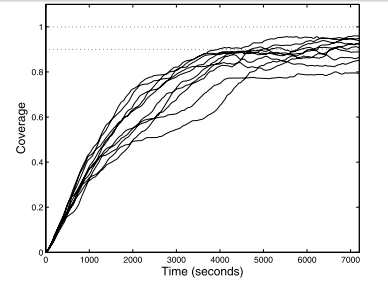
\includegraphics{../images/random_coverage.png}
   \caption{\label{randomcoverage} Random mobility coverage\cite{UAV}}
\end{figure}

\newpage

\begin{figure}[!h]
   \centering
   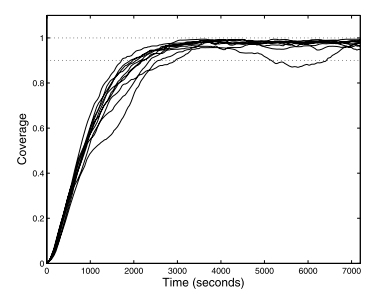
\includegraphics{../images/pheromone_coverage.png}
   \caption{\label{pheromonecoverage} Pheromone mobility coverag\cite{UAV}}
\end{figure}

For the random model, we see that it need more than 83 minutes to reach 80 percents of coverage. Whereas the pheromone model reach the 90 percents in 60 minutes. Comparing the two models, the pheromone model has a much higher coverage rate.

\subsection{Scan Characteristic}

In Figure \ref{randomchar} and Figure \ref{pheromonechar}, the solid lines represent the probability distribution of each models. This curve permits to calculate the probability of the next scan.\\
To know the probability of the next scan between the time t1 and t2, we have to calculate the area under the curve between t1 and t2.\\
So to meet with the requirement of one scan of the map per hour, the curve must be 0 at 1 hour. However none models reach 0 before one hour, because no model manages to achieve full coverage, the pheromone model manages well to avoid rescanning a recently scanned area. We can see that on the graphic : the median curve follows the dashed line at time between 0 seconds and 1000 seconds.

\newpage

\begin{figure}[!h]
\centering
   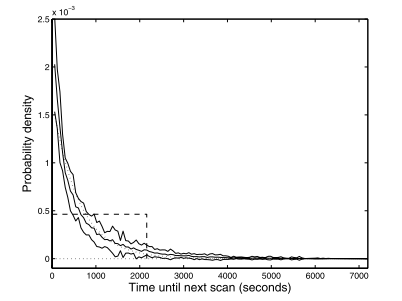
\includegraphics{../images/random_scan_characteristic.png}
\caption{\label{randomchar} Random mobility\cite{UAV}}
\end{figure}

\begin{figure}[!h]
   \centering
   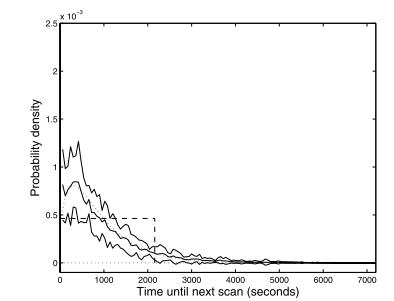
\includegraphics{../images/pheromone_scan_characteristic.png}
\caption{\label{pheromonechar} Pheromone mobility\cite{UAV}}
\end{figure}

\subsection{Never scanned area}

In this table below, we can see the results about the percentage of the map never scanned.\\

\begin{center}
\begin{tabular}{|c|c|c|c|}
\hline
	      & Max & Median & Min \\
	      \hline
	Random & 16.2\% & 3.2\% & 0.5\% \\
	\hline
	Pheromone & 0.21\% & 0.03\% & 0.01\% \\
	\hline
\end{tabular}
\end{center}

It represents the maximum, median and minimum uncovered area for the ten runs. These numbers clearly show the ability of the pheromone model to cover the complete area. 

\newpage

\subsection{Connectivity}

\begin{figure}[!h]
   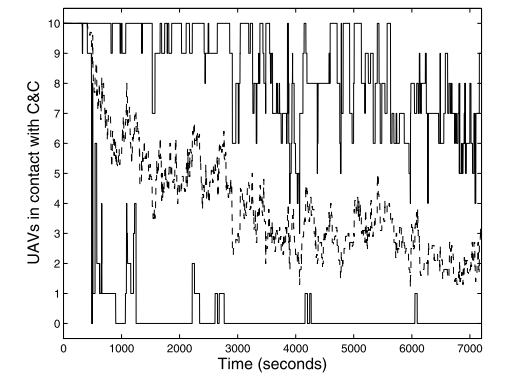
\includegraphics{../images/random_resultat_connectivite.png}
\caption{\label{randomconnect} Random. Number of UAVs in contact with C\&C (max, average, min)\cite{UAV}}
\end{figure}

\newpage

\begin{figure}[!h]
   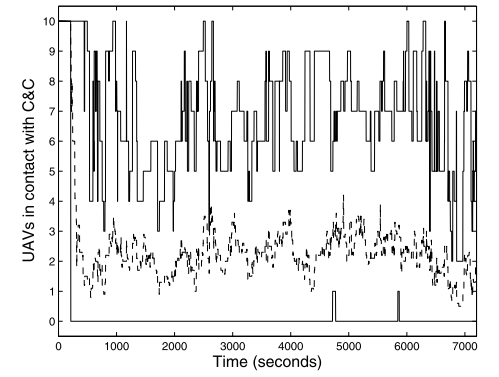
\includegraphics{../images/pheromone_resultat_connectivite.png}
\caption{\label{pheromoneconnect}Pheromone. Number of UAVs in contact with C\&C (max, average, min)\cite{UAV}}
\end{figure}

In Figure \ref{randomconnect} and Figure \ref{pheromoneconnect},we can see the number of UAV wich can communicate with the C\&C.  The  graphs  show the maximum, average, and minimum of this number for the ten runs. We saw that both models don't provide good connectivity. There are not enough UAV to have a fully connected communication graph. Because of the pheromone logic that pushes the UAVs away from each other, this model have low connectivity. Whereas the random model have a high connectivity at the beginning of the run. Then with the random trajectory of each UAV, they move away from each others and finally this model finishes to have the same poor connectivity as the pheromone model.

\section{Our Implementation}

\subsection{Scan coverage}

The graphic \ref{scancoverage} is the result of our experiments using our implementation of the random walk and waypoint mobility model and the pheromone mobility model. Each run lasts 20 minutes and uses 10 UAVs per model. (compléter éventuellement avec le C and C).

\begin{figure}[!hbtf]
\centering
   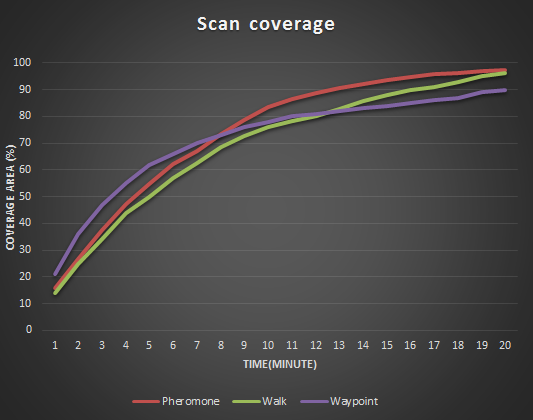
\includegraphics{../images/ScanCoverageResult.png}
\caption{\label{scancoverage} Scan coverage resulting of our implementation}
\end{figure}

\begin{itemize}

\item Observation

We can see that the random waypoint mobility model covers a higher scan area until 7 minutes than the others mobility models. From 7 minutes to the end, the better mobility model is the pheromone one. The random walk is in third position until 13 minutes, at this time, this is the random waypoint becomes the third. At the end of the run, the random waypoint doesn't exceed 90\%, the random walk rises approximatly to 95 \% and the pheronome model a little bit.

\item Interpretation

The random waypoint is better to reach a higher percent of scanned area because each UAV chooses a destination and travels to. But at a moment, the most part of the time, the UAVs pass again on an area already scanned. Hence the random waypoint can't target 100\% in a reasonable time.

The random walk is slower than the others models because each UAV changes its destination each second. But at the end of the simulation, this model reaches over 90\% like the pheromone model. Indeed, this model takes a long time to disperse each UAV all over the map.

The pheromone model quickly distributes all the UAVs over the map because the UAVs repel others. So this model is more efficient than the random walk. But, at the beginning of the run, the random waypoint is more efficient than pheromone model because this one include a part of random mobility model in the moving of each UAV. Each of them change its direction every second. Finally, the percent of scanned area increases progressively.

\item Conclusion

The pheromone mobility model is the better model to reach quickly the most percentage of scanned area. Indeed, the random mobility models aren't appropriate to scan the entire area.


\end{itemize}


\subsection{Connectivity}


